\chapter[Comptage haut débit de populations en
microcosmes élevées au laboratoire][Comptage haut débit]{Comptage haut débit de populations en
microcosmes élevées au laboratoire}

\begin{Spacing}{1}
\texttt{
Mallard, François, Vincent Le Bourlot, and Thomas Tully. "An Automated Image
Analysis System to Measure and Count Organisms in Laboratory Microcosms." PLoS
One 8, no. 5 (2013)
} 
\end{Spacing}

\section*{Abstract}
\addcontentsline{toc}{section}{Abstract}

%\begin{enumerate}
%\item 
\lettrine[lines=3]{B}{ecause of} recent technological improvements in the way
computer and digital camera perform, the potential use of imaging for contributing to the study of
communities, populations or individuals in laboratory microcosms has risen
enormously. However its limited use is due to difficulties in the automation of
image analysis.
%\item 

We present an accurate and flexible method of image analysis for detecting,
counting and measuring moving particles on a fixed but heterogeneous substrate.
This method has been specifically designed to follow individuals, or entire
populations, in experimental laboratory microcosms. It can be used in other
applications.
%\item 

The method consists in comparing multiple pictures of the same experimental
microcosm in order to generate an image of the fixed background. This background
is then used to extract, measure and count the moving organisms, leaving out the
fixed background and the motionless or dead individuals.
%\item 

We provide different examples (springtails, ants, nematodes, daphnia) to show
that this non intrusive method is efficient at detecting organisms under a wide
variety of conditions even on faintly contrasted and heterogeneous substrates.
%\item 

The repeatability and reliability of this method has been assessed using
experimental populations of the Collembola \textit{Folsomia candida}.
%\item 

We present an ImageJ plugin to automate the analysis of digital pictures of
laboratory microcosms. The plugin automates the successive steps of the analysis
and recursively analyses multiple sets of images, rapidly producing measurements
from a large number of replicated microcosms.
%\end{enumerate}

\section{Introduction}

Because of their relatively short generation time and ease of rearing,
invertebrate species are ideal for studying population dynamics and life history
traits: \textit{Daphnia} \autocites{drake2009a,hebert1978a}, Drosophila
\autocites{mueller2005a}, mites \autocites{benton2005a}, Collembola
\autocites{tully2008a,pike2004a}, Nematodes \autocites{alvarez2005a,chen2001a}.
But even in these convenient model organisms, data collection is often made by
eye which is possible when populations are very small
\autocites{pike2004a,drake2004a}, but can soon become far too time consuming.

Measurements can be made using digital images of individuals or populations.
Pictures are ideal because they are taken rapidly, they are innocuous, cheap and
can be stored and re-observed if necessary. During the past fifteen years, the
technological improvements of digital cameras, hard drive storage capacities and
computer performances \autocites{walter2005a} has radically changed the way
researchers use images to collect and store information on their experiments..
Numerous image analysis software are now available \autocites{eliceiri2012a} many of which
are open-source \autocites{schneider2012a}. In experimental ecology, such progresses
enables the acquisition of large amounts of pictures and the tracking of individual behaviour, fecundity or growth
trajectory on a fine time scale and over long periods of time. The measurement
itself can be made manually on a computer using appropriate image analysis
software such as ImageJ \autocites{schneider2012a,abramoff2004a} to estimate egg
and body sizes for instance \autocites{tully2008a,plaistow2009a}. Massive image
capture and analysis can also be used to follow the size and structure of an experimental population. But even on pictures, measurements
remain time-consuming and may quickly become impractical. Reliable and
reproducible automatic counting and measuring methods are then needed.
Various authors have designed and proposed image analysis methods to
automatically measure or count small organisms in the laboratory
\autocites{hooper2006a,krogh1998a,auclerc2010a,lukas2009a,marcal2006a}.
But these methods fail at dealing with heterogeneous substrates and the particles
and dead individuals that are prone to be detected as living individuals in the
automatic census. Here we present a simple image processing method that can
increase the efficiency and reliability of particle detection and population
monitoring which has seldom been used before in ecology
\autocites{faerovig2002a,mallard2012a}.
The principle used here is based on the particle analysis developed in the ImageJ
multi-tracker plugin \autocites{kuhn2001a}. The idea is to compare several pictures
of the studied microcosm to construct a composite picture made  up from the motionless
elements. This will generate a background image which can then be removed from
the original pictures to show only the elements that moved, which are often the
organisms being studied. It requires simple material (a digital camera or a
webcam, a stand and a good lighting device) and an image processing program.
Here we used the open-source ImageJ software \autocites{abramoff2004a}.

We first describe the different steps of the image segmentation using a
laboratory population of the springtail \textit{Folsomia candida} (Collembola,
Isotomidae) as a model microcosm \autocites{fountain2001a}. The same method is
applied using different environments to illustrate the variety of biological models and
questions that can be tackled with it. We then give some quantitative
assessments of the method’s reliability and robustness using again the
collembolans as a case study. Finally, we describe an ImageJ plugin that we have
developed to automate batch laboratory population census.

\section{Materials and methods}

\subsection{Method overview}

\subsubsection{Image acquisition}

The first step is to take a set of pictures (usually from three to five) of the
microcosm being studied with constant framing and lighting (Figure \ref{Fig21-1}a). The
camera and the microcosm have to be kept in exactly the same position while the
stack of pictures are taken. We used a digital camera fixed on a stand and
remotely controlled by a computer (Nikon D300 and CameraControlPro). Constant,
homogeneous and strong lighting was provided by four LED bulbs (Pikaline, 16W,
650 lumens). It is always better to have a good light homogeneity but, as
discussed below, the method can compensate for partial lighting inhomogeneity.
Temporal stability of lighting conditions between pictures in a stack is more
important. Using fluorescent lamps is not recommended since their light
intensity varies, causing lighting heterogeneity between pictures. We also
recommend not to use incandescent light bulbs as they produce a lot of heat that
can perturb or harm the studied organisms.

\begin{figure}[!ht] % Figure 1 
\centering
\includegraphics[height=0.75\textheight]{2_Methodo/Fig/1_collemboles_etapes.pdf}
\caption[\lofimage{2_Methodo/Fig/1_collemboles_etapes.pdf} The successive steps
of the image analysis]{The successive steps of the image analysis. (a) Two of
the original pictures of a population of Collembola \textit{Folsomia candida} raised on humid plaster of Paris darkened with Indian ink. (b) The constructed still background picture.
Each pixel is calculated as the darker pixel of the original set of pictures.
(c) Subtracting (b) from (a) removes the still background and reveals the
springtails. The white grain in the background (see arrow) has disappeared. (d)
After thresholding it becomes possible to count and measure the springtails with
great confidence.
}
\label{Fig21-1}
\end{figure}

\subsubsection{Creation of a background picture}

Using ImageJ, the pictures are put into a stack (menu File, Import, Image
Sequence) and then compared (Image, Stacks, Zproject) to generate a new image
composed of all the elements that remained motionless (Figure \ref{Fig21-1}b). Each pixel in
the stack is analysed and at each position only the one of minimal intensity (i.
e. the darkest one) is kept. Other methods (median, mean) are recommended if the
picture quality is heterogeneous or if the pictures are taken on a time scale
long enough for the lighting conditions to vary slowly. The resulting image -
the still background - is then subtracted from each of the original stack
pictures (Process, Image Calculator, Figure \ref{Fig21-1}). This produces a new stack of
images that only contains the mobile elements, here the collembolans (Figure
\ref{Fig21-1}c).

\subsubsection{Detecting, measuring and counting the organisms}

The next step is the thresholding procedure that will transform the 8-bit
images (256 grey levels) into black and white 2-bit images (Image, Adjust,
Threshold, Figure \ref{Fig21-1}c). The selected threshold value determines the grey level
above which the pixels will become white and under which they will become black
and be measured. Removing the substrate image created a homogeneous background,
on which the organisms are clearly visible. Particle measurement becomes less
sensitive to the chosen threshold value, since a large range of threshold values
gives equivalent results. Once the 2-bit pictures are created, the ImageJ
"Analyse Particles" function can be used to count and measure the particles.

\subsection{Application examples from various biological systems}

To prove the wide potential use of this method in experimental ecology, we
worked on several other biological systems. In the first two, we counted and
measured other model organisms in their usual laboratory environments (nematodes
in agar plate and zooplankton in a pond sample). We then give two other
methodological applications: the tracking of a single collembolan and the
measurement of ants’ activity during a long period of time. No endangered or
protected species were involved and no specific permission was required. The
animals were just briefly used for taking a set of pictures without being harmed
by handling them.

\subsubsection{Detecting and counting nematodes in a Petri dish}

This method was tested for detecting nematodes (Caenorhabditis elegans) on agar
in a Petri dish (Figure \ref{Fig21-2}a). We took a set of 10 pictures interspaced at
approximately 5 to 10 sec. We used the same camera as previously and the Petri
dish were lit up from below using the lighting device of a dissection
microscope.

\begin{figure}[!ht] % Figure 2 
\centering
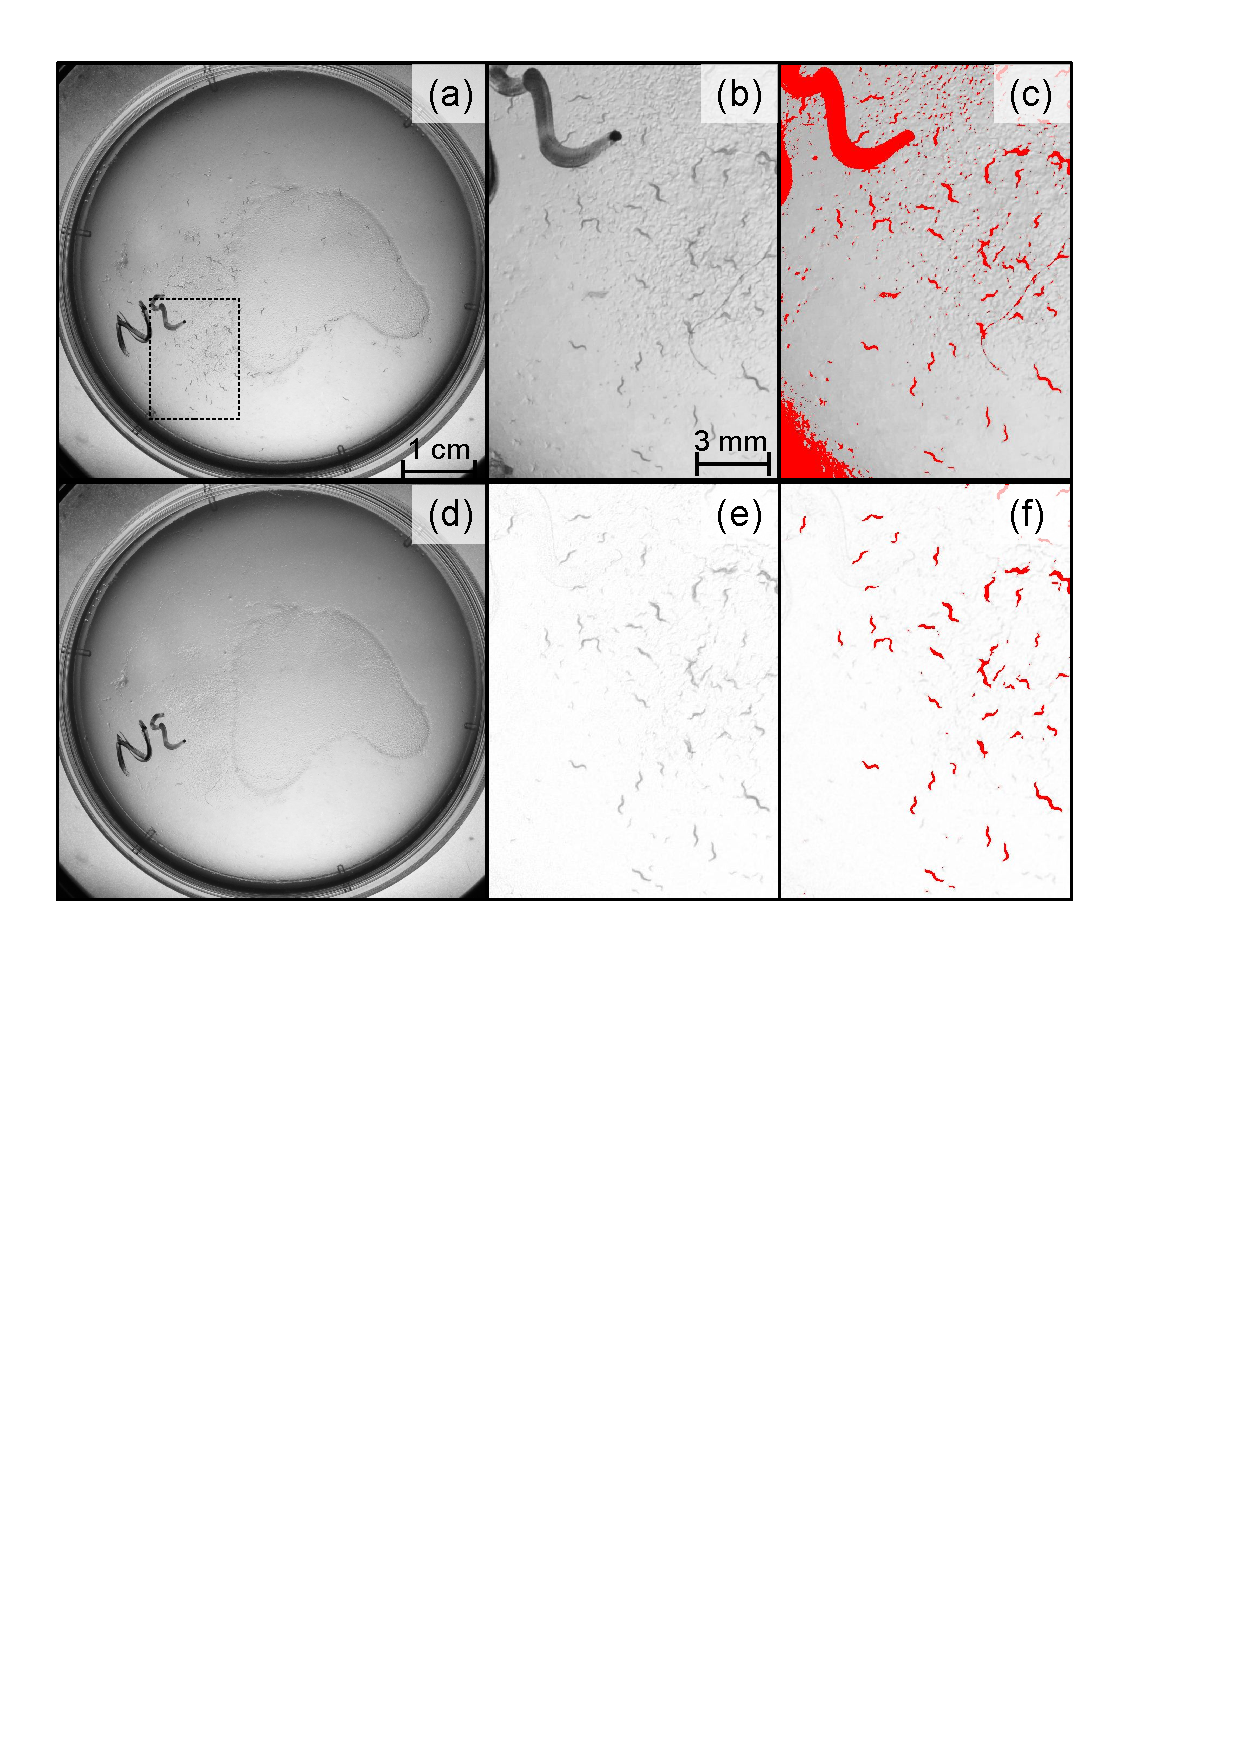
\includegraphics[width=0.95\textwidth]{2_Methodo/Fig/2_Nematodes.pdf} 
\caption[\lofimage{2_Methodo/Fig/2_Nematodes.pdf} Detecting nematodes on agar in a Petri dish]{
Detecting nematodes on agar in a Petri dish. Several pictures of a standard
nematode rearing plate such as (a) have been taken. From this stack of pictures,
a background image (d) has been created. The four other panels are close-up
views of the same area (dashed rectangle of (a)) before (b, c) and after (e,f)
the removal of the background image. A standard particle analysis run on the
original pictures (b,c) failed to bring out only the nematodes: an optimal
thresholding is impossible because of the background heterogeneity (c). But
removing the still background (e) allows a much more efficient detection of the
nematodes (f).}
\label{Fig21-2}
\end{figure}

\subsubsection{Counting and identifying pond copepods and ostracods}

The method has also been applied for detecting zooplankton (\textit{Daphnia} \&
\textit{Cypris}) in a sample of pond water containing some filamentous algae
(Figure \ref{Fig21-3}a,b). We used the same camera and lighting unit as in the case of the collembolan population.
In order to generate the background image five coloured pictures (interspaced at
app. 5 to 10 sec) have been compared (Figure \ref{Fig21-3}c).

\begin{figure}[!ht] % Figure 3 
\centering
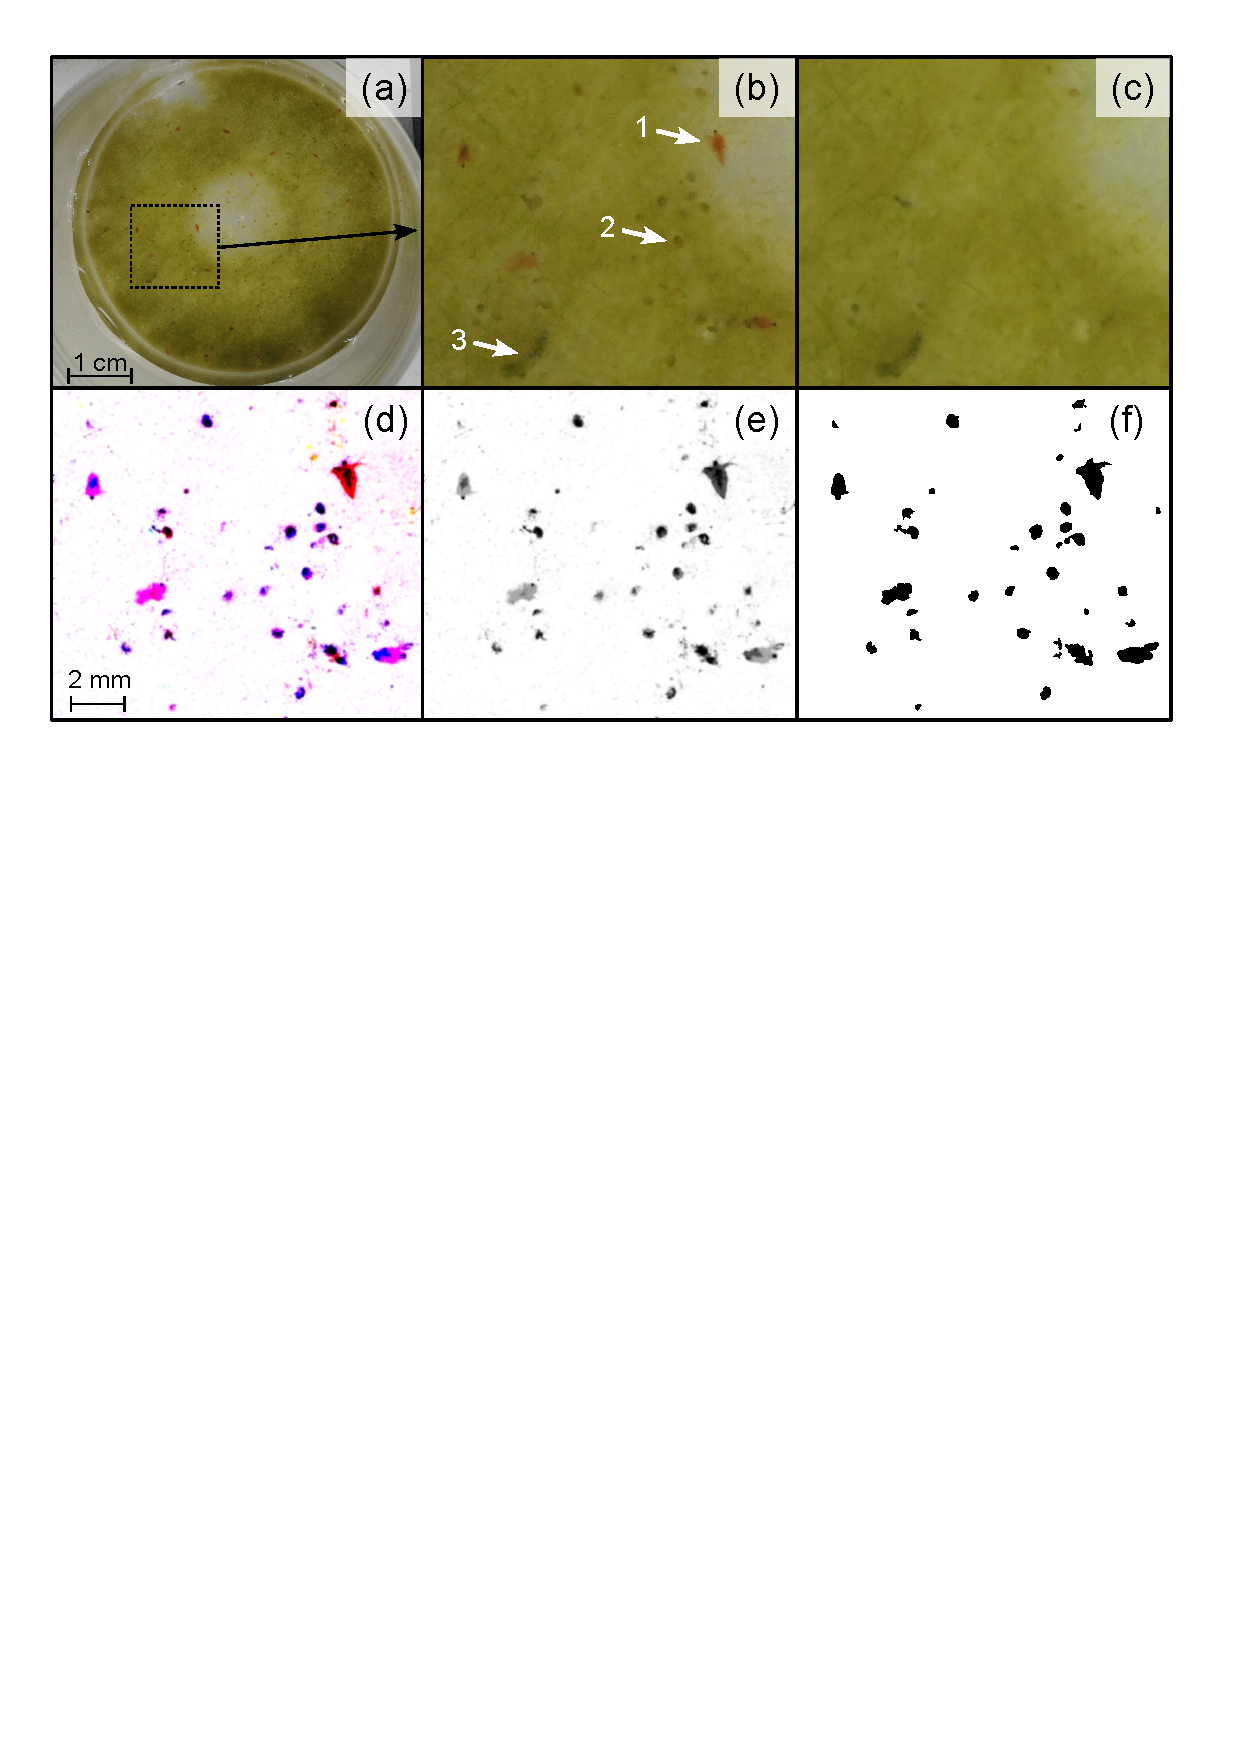
\includegraphics[width=0.95\textwidth]{2_Methodo/Fig/3_Daphnies.pdf} 
\caption[\lofimage{2_Methodo/Fig/3_Daphnies.pdf} Detecting and counting the zooplankton in a sample of pond water]{ Detecting and counting the zooplankton in a sample of pond water. (a) One
picture among five similar ones. (b) A close-up view (dashed rectangle) reveals
a few Cladoceran (red \textit{Daphnia}, arrow 1) and several small Ostracods (\textit{Cypris} sp.,
arrow 2) on a layer of green algae. The difference between (b) and still
background (c) reveals the particles that have moved, i.e. the crustaceans. This
picture can be transformed into an 8-bit grey image (e) which can be used to
detect, measure and count the zooplankton (f). The immobile dark clumps (arrow
3) are excluded from the census. The colour image (d) can also be used to
identify different species.}
\label{Fig21-3}
\end{figure}

\subsubsection{Tracking the movements of an isolated collembola}

In this example, we put a single collembola into a container made of three
connected square compartments filled with a substrate of humid and darkened
plaster and track its exploratory behaviour (Figure \ref{Fig21-4}). Two hundred pictures of
the box were taken, one every 5 sec. The lighting unit used was similar to that
previously described for the collembola system.

\begin{figure}[!ht] % Figure 4 
\centering
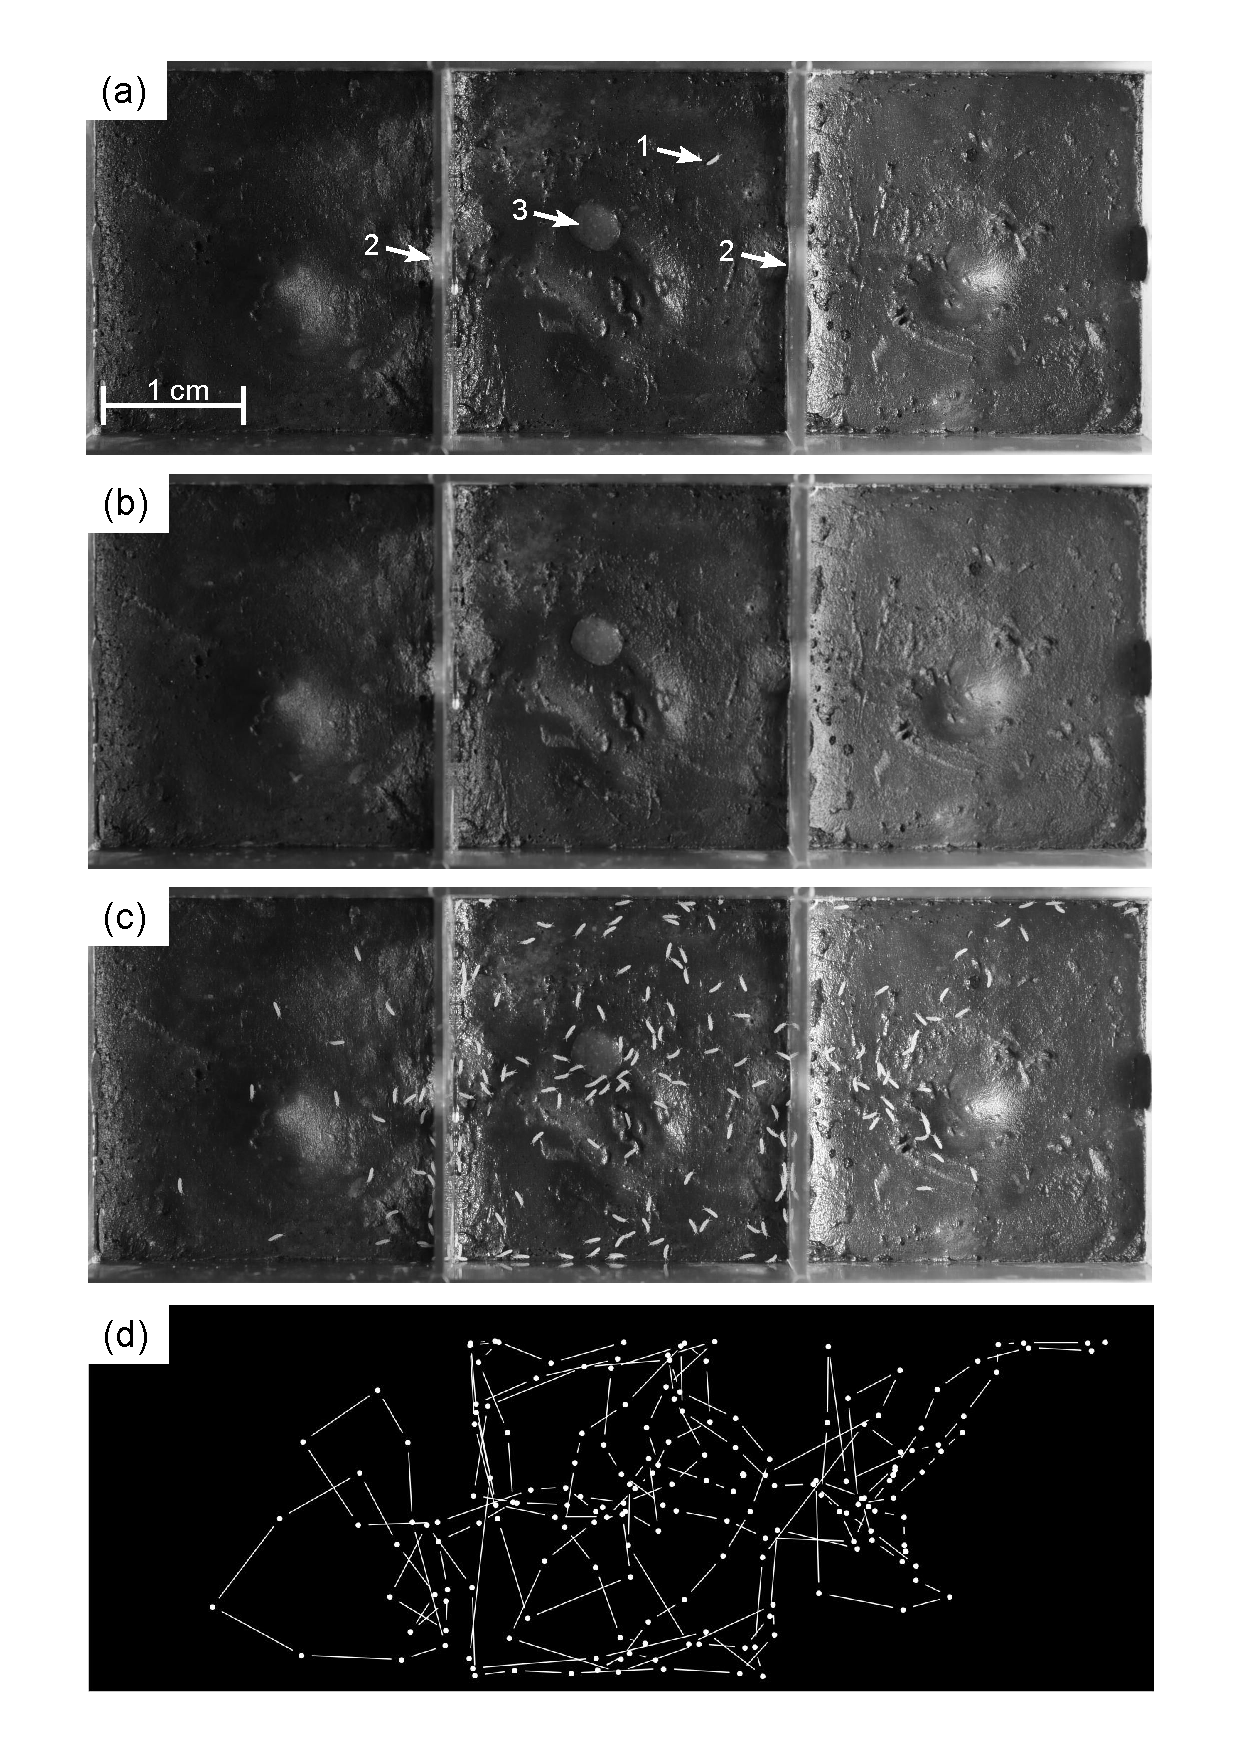
\includegraphics[height=0.75\textheight]{2_Methodo/Fig/4_TrackCollemboles.pdf}
\caption[\lofimage{2_Methodo/Fig/4_TrackCollemboles.pdf} Tracking an isolated collembolan wandering in a container]{ Tracking an isolated collembolan wandering in a container. The container is made of three compartments connected by small holes (arrows 2). A
pellet of food (arrow 3) is visible. A picture was taken every 5 sec. during 30
min. The still background (b) was calculated by averaging the 300 pictures. It
was then then subtracted from each picture to reveal the collembolan. Picture
(c) is the addition of the background (b) and of all the images after the
background's removal. It shows the different positions of the collembola during
the follow-up. The full track of the springtail is plotted on panel (d).}
\label{Fig21-4}
\end{figure}

\subsubsection{Measuring the temporal dynamics of activity in an ant colony}

A high resolution usb webcam (Dinolite AM7013MZT, 5 Mp) was placed above a
laboratory ant colony (Figure \ref{Fig21-5}a) continuously lit by a LED bulb. The camera was
programmed to capture an image of the nest entrance (Figure \ref{Fig21-5}, arrow 1) every 30
sec during 18 hours. The $\approx$2000 images have then been processed with ImageJ in
order to compute the fixed background. The number of ants wandering around the
nest were then automatically counted on each picture (Figure \ref{Fig21-5}d).

\begin{figure}[!ht] % Figure 5 
\centering
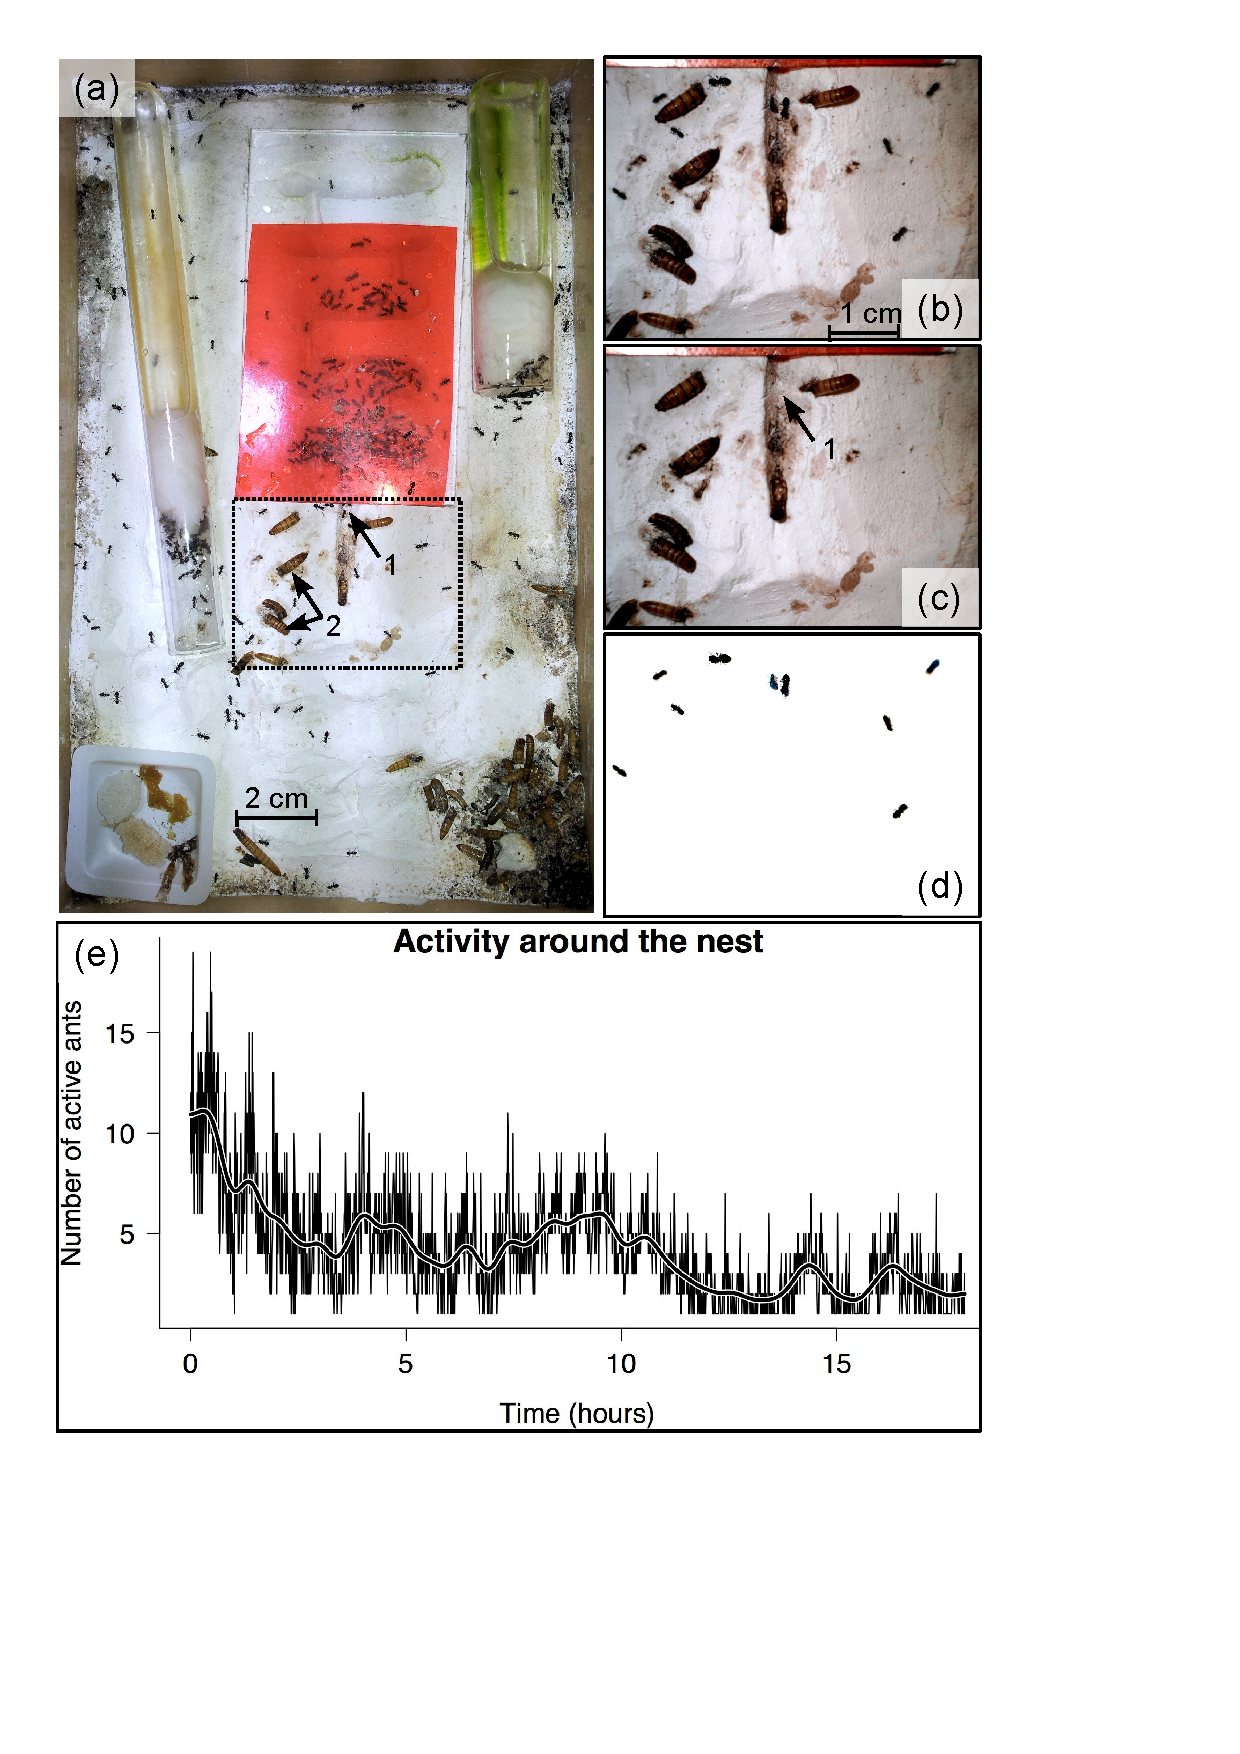
\includegraphics[height=0.60\textheight]{2_Methodo/Fig/5_Fourmis.pdf} 
\caption[\lofimage{2_Methodo/Fig/5_Fourmis.pdf} Follow-up of the activity of an ant colony]{ Follow-up of the activity of an ant colony. (a) General view of an ant colony
bred in the laboratory on a plaster substrate. The below-ground colony is under
the red plastic slate. The ants activity around the nest entrance (arrow 1) has
been followed within the dashed rectangle (b). (c) The background image is built
up through the comparison of multiple pictures (median value). (d) The
difference between (b) and (c) reveals the ants entering and exiting the nest.
Immobile dark particles such as remains of food (Tenebrio larvae, arrow 2) are
discarded from the analysis. (e) By automatically repeating the previous steps,
one can easily count the number of active ants around the entrance of the nest.
This has been done every 30 sec for 18 h. The graph displays all these
measurements and reveals the temporal dynamics of the mean activity around the
nest.
}
\label{Fig21-5}
\end{figure}


\subsection{Method reliability}

\subsubsection{How many pictures are needed ?}

We studied the minimal number of images needed according to particle density,
using springtail populations as an example (Figure \ref{Fig21-1}). We took sets of twenty
pictures of ten rearing boxes with increasing densities of juveniles measuring
$\approx$0.15 to 0.5 mm long. For each density, we performed our analysis on different
subsets of the whole set of pictures, progressively increasing the number of
images used to calculate the background (Figure \ref{Fig21-6}a). A total of 320 sets of
pictures were analysed.

\begin{figure}[!ht] % Figure 6 
\centering
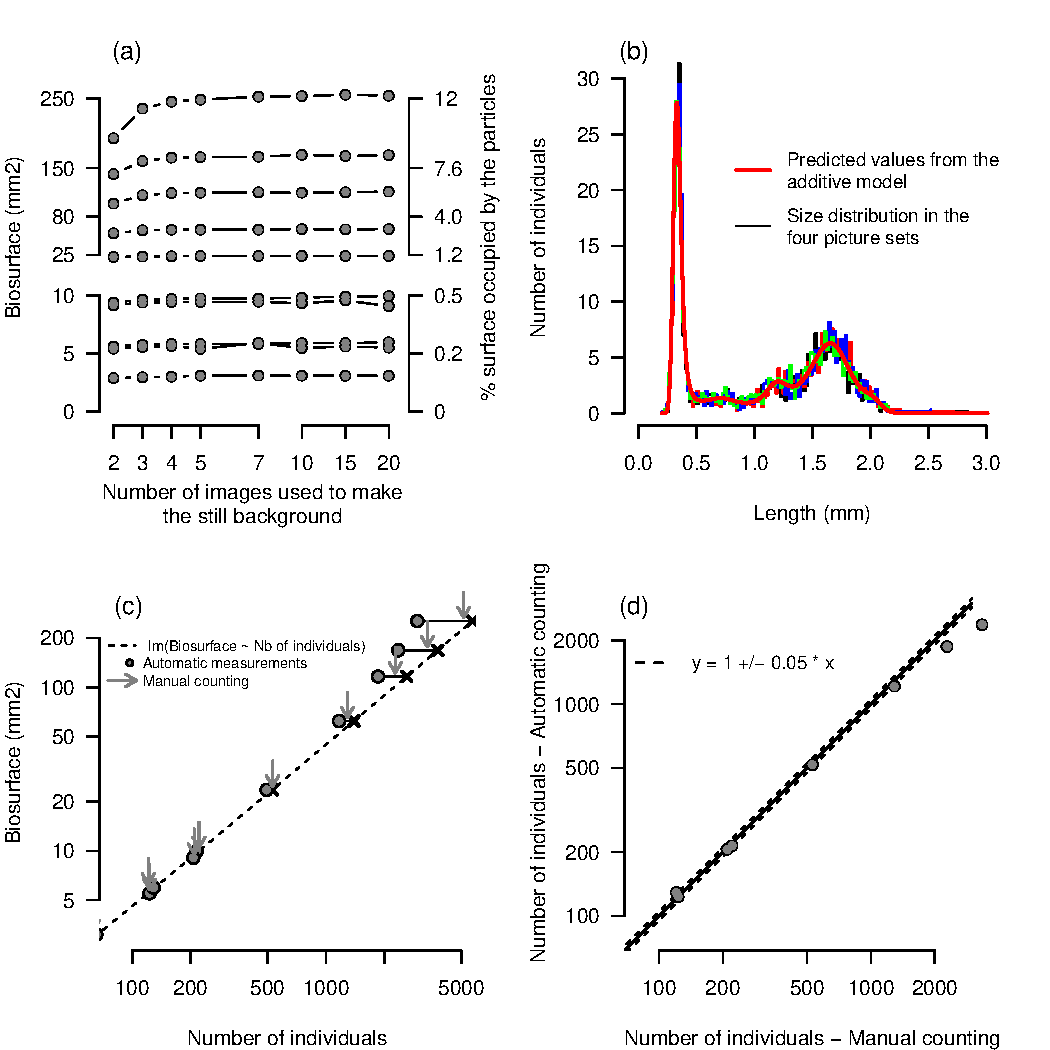
\includegraphics[width=0.90\textwidth]{2_Methodo/Fig/6_Plugin_multiP.pdf}
\caption[\lofimage{2_Methodo/Fig/6_Plugin_multiP.pdf}  Assessing the method's reliability on a collembola population]{ Assessing the method's reliability on a collembola population. (a) Total measured collembolan biosurface (mm2) depending on the number of pictures
in the stack. For low densities, two or three pictures are sufficient to have a
good and reliable measurement. For higher densities, four or five pictures are
needed. (b) Size distribution of the same collembola population. Four different
sets of pictures taken by two different users were analysed. The size classes
are 0.02 mm width. We fitted a generalised additive model that did not show any
significant difference between the pictures nor between the sets. (c-d)
Reliability of the automatic counting method. (c) The estimated biosurface
measured in 10 boxes and the number of individuals automatically counted
(circles). Results of the manual counting are shown (grey arrows) together with
a linear regression between the biosurface and the number of individuals
calculated for the five lowest density boxes. (d) Comparison of the number of
individuals for automatic and manual counting methods.
}
\label{Fig21-6}
\end{figure}

\subsubsection{How repeatable are the measurements of a population structure?}

To illustrate the repeatability of the method for measuring a population
structure, we analysed four sets of five or six pictures of the same collembolan
population (Figure \ref{Fig21-6}b). We divided the size distribution of collembolan (from
0.1 to 3 mm) into 145 classes, each of 0.02 mm width, and analysed the number of
individuals in these classes using a generalised additive model (GAM, function
gam of the mgcv library in R) with a Poisson distribution, a cubic regression
spline, and an imposed high number of knots (k=20) to fit the data closely. We
then tested differences between the pictures and the stacks of images using
anova and Chi-squared tests.

\subsubsection{Are the counting measurements reliable?}

To test whether our counting method is reliable, we compared - for several
collembolan densities - the number of particles automatically counted using the
background removal method with a measurement made manually. Ten sets of 20
pictures each were analysed automatically to measure the mean number of
particles and their total surface. The number of individuals was also measured
manually on one picture belonging to each set (Figure \ref{Fig21-6}c-d). We then performed a
linear regression between the surface and the number of individuals calculated
for the five lowest density boxes. The analyses were all implemented in R 2.15.2
software (\url{http:// cran.r-project.org}, \citealp{ihaka1996a}).

\subsection{Automated implementation}

We present an ImageJ plugin called BP\_sensor for “Batch population sensor” that
we have developed to automate the measurements of size and structure in many
replicated laboratory populations raised in experimental microcosms (Figure \ref{Fig21-S1}
in Section \ref{21-SM1}). This plugin was specifically designed to track populations of the
Collembola \textit{Folsomia candida} but it is versatile enough to be easily adapted to
other experimental setups (Figure \ref{Fig21-S2} in Section \ref{21-SM1}). It automatically performs the
recursive census of multiple laboratory populations of collembolans (Figure \ref{Fig21-S3}
in Section \ref{21-SM1}). The code is written in Java and runs within the freely available
and open-source ImageJ software (\citealp{abramoff2004a}, 
\url{http://rsbweb.nih.gov/ij/}).
% We
% provide in the Supporting Information the commented Java code (File S2) that can
% be directly compiled and run with ImageJ as well as a set of image examples
% (File S3) and some explanations (Section \ref{21-SM1}) to help understand how it works and
% how it can be customised (see Table \ref{Tab21-1} in Section \ref{21-SM1}).

\section{Results and discussion}

\subsection{Counting and tracking individuals in various biological systems}

The method we propose allows a standardisation and automation of microcosm
measurements. The segmentation of pictures into regions of interest that match
structural units is one of the most critical steps in the process of reducing
the complexity of images and extracting information \autocites{russ2002a}. It
usually relies on efficient and precise thresholding. When a single picture is analysed without
making use of our background removing procedure, the efficiency of this crucial
thresholding step can be improved by (1) controlling the overall luminosity to
ensure selecting particles with the same precision everywhere on the picture
(homogeneous lighting) and by (2) maximising the contrast between the particles
(here living organisms) and their background (here substrate) to get a straight
particle segmentation. Removing the motionless background corrects for
heterogeneity in lighting conditions and in the underlying substrate. In Figure
\ref{Fig21-4}, the blackness of the substrate is heterogeneous on the original
pictures which would hinder a standard particle analysis to operate efficiently. This
background removal method is also a way to suppress motionless particles and to
increase the contrast between moving particles and their substrate (Figure
\ref{Fig21-1}c,f). It then becomes possible to automatically adjust the
threshold value required for particle measurements since a larger range of the thresholding values will give similar results.

This increased robustness comes at a cost: the multiple pictures have to be
perfectly lined up. Even a slight movement can blur the constructed background
image and the rest of the analysis will fail. That is why we recommend using a
stable stand and a remote shutter release to avoid any movement of the camera.
Note that it is possible to translate and re-align images that have moved using
the multiplication of the Fourier transformed images (convolution). Our method
is also sensitive to temporal luminosity variations: the moving particles can
create shadows that darken their surrounding substrate, which locally reduces
the efficiency of the background removal. Providing omnidirectional and stable
lighting limits the formation of shadows and easily avoids these unwanted
effects.

On 8-bit grey images, the background image can either be calculated as the
maximum or the minimum grey value in the stack, depending on whether the moving
particles are lighter or darker than their substrate. In our case study, the
springtails are lighter than the darkened plaster and we used the minimal value.
However, using the median or the mean value can be advantageous, especially when
the background is very heterogeneous or the contrast between the particles and
the substrate is so small that the moving elements can be either darker or
lighter than the substrate depending on their positions. For these reasons, we
used the mean grey value to calculate the background in all four additional
examples. To be efficient, the number of analysed and compared pictures has to
be relatively high (at least 4 or 5). Similarly, it is often more efficient to
remove the background by computing the “difference” between the original images
and the background rather than simply the “subtraction” (see the options of the
ImageJ “Image calculator” function). Here we applied this method to extract the
nematodes from their background as they were either brighter or darker than
their agar substrate, depending on the local light reflection.

Given a few adjustments, our measurement method can be applied to various
systems. It was quite efficient at highlighting nematodes on agar. Removing the
background (Figure \ref{Fig21-2}d) improved the reliability for the detection of nematodes
(Figure \ref{Fig21-2}b,c and f) even though the image was faintly contrasted (Figure \ref{Fig21-2}e).
Although it improved the detection of adults, the analysis was not perfect
since, for example, the small worms were not detected (Figure \ref{Fig21-2}). But the use of
a more performant and homogenous lighting unit, combined with some additional
image processing such as smoothing, could certainly improve the analysis
efficiency.

In the pond water sample (Figure \ref{Fig21-3}), the “substrate” is not motionless: the
swimming organisms can shake or move the algae or non living fragments floating
around, which can alter the process of background removal. But despite this
potential drawback, the method turned out to be pretty efficient at bringing out
the zooplankton. It even managed to reveal minor morphological details which
were almost hidden in the original pictures (cf. antenna of the \textit{Daphnia} pointed
by arrow 1 on Figure \ref{Fig21-3}c). However, long term tracking (as for the ant colony or
an isolated springtail) would probably fail owing to too much long term blurring
of the background – unless several backgrounds are recursively constructed on a
shifting subset of the whole stack of images.

Figure \ref{Fig21-4} illustrates how this method can be used to easily track the movement
and behaviour of an individual exploring an heterogeneous landscape (cf.
multi-tracker plugin \citealp{kuhn2001a}). The ant activity around the nest is
also an interesting application example. We did not track through time a constant number
of moving particles nor census a complete population but counted individuals in
a partial area of the colony on a long time scale (18h). The entire data were
then grouped on a diagram in order to show the temporal dynamics of the colony’s
activity near the nest entrance (Figure \ref{Fig21-5}). We do not compare the results
obtained with manual measurements that would be very time consuming. However,
the activity measurements are coherent with an initial increased activity, no
doubt caused by disturbance during the setting up of the experiment (Figure \ref{Fig21-5}e):
the second half of the measurements were done at night and this could explain
the decrease of activity.

For both the pond water sample (Figure \ref{Fig21-3}) and the ant colony (Figure \ref{Fig21-5}), the
processing was done on coloured pictures. This provided interesting additional
information since the colour remained after removal of the background. This
information could be used together with the size and shape of the particles to
help identify, for instance, different species (here \textit{Daphnia} \& \textit{Cypris}, Figure
\ref{Fig21-3}d). Such colour images could also benefit from some specific
treatment such as decorrelation stretch (DStretch imageJ plugin) to bring out the different
particles of interest \autocites{harman2011a}.

\subsection{Testing the method’s reliability in an optimised acquisition system}

\subsubsection{Background calculation - Number of pictures needed}

The reliability of the method relies on the quality of the still background
image, which has to be free from any moving particle. This will depend on the
number of images compared to make the background and on the proportion of the
substrate occupied by the creatures. If their density is high, more images are
needed for each pixel of the substrate to be visible on at least one image. The
replicated analysis performed with increasing number of images in a single stack
showed that the total measured biosurface increases with the number of pictures
analysed (Figure \ref{Fig21-6}a). But for low densities (0 to 250 individuals - which
corresponds to a biosurface of 3 to 10 mm2, the rearing box surface measuring 20
cm2), this increase is almost negligible. For these low densities, the
probability that part of the substrate is covered by a collembola on more than
one picture is very low. Taking more than two pictures does not really improve
the reliability of the measurements. But for higher densities, three, four or
five pictures are needed to reveal the whole background substrate which is
needed for reliable and robust estimation of the population biosurface. In our
study case, taking more than five pictures never improved the measurement
reliability. As a rule, comparing four pictures ensures reliable measurements.

\subsubsection{Repeatability of a population structure measurement}

The estimation of the population structure was repeatable (Figure \ref{Fig21-6}b): the four
estimated size distributions were largely overlapping. A fitted generalised
additive model to these distributions explains most of the variance (84\%) and
we found that the estimated size distributions did not differ between the
different sets of pictures ($\gamma ^2_3$=2.3, p=0.5), nor between the different
pictures within each set ($\gamma^2_{22}$=23.2, p=0.4).

\subsubsection{Reliability of the counting measurement}

The reliability of automatic measurements is good for densities below 1000
individuals, but beyond this density the automatic counting underestimates the
density (controlled manually):  more and more individuals adjoin each other and
are then detected as one large particle (Figure \ref{Fig21-6}d). The measured total
biosurface then becomes a better proxy for the number of individuals in the box:
a projection of the biosurface values of the five highest densities on the
linear regression provides a less biased density estimate (Figure \ref{Fig21-6}c). But this
correction only works if the individuals have similar size and if they do not
overlap, which is the case here. A more complex particle image analysis, like
the watershed algorithm \autocites{vincent1991a} could also be used to split up
merged individuals.

\subsection{Automated implementation}

We have developed an automatic measuring and counting procedure using multiple
picture analyses that is easy to use and requires very few calibrations (see
ESM). It takes about two hours to obtain five pictures of a hundred populations
and to manually sort these pictures in a normed directory tree on the computer.
It then takes about one hour for the plugin to analyse these 500 images, count
and measure all the individuals in these populations and save the data in
distinct files (20 to 30 sec per set of 5 pictures on a 2.5GHz computer).
Altogether about three hours are needed to take a census of one hundred
laboratory populations, whose densities can reach a thousand individuals.

One of the major improvements would be to use colour pictures instead of black
and white ones. It would not change the background image calculation but would
allow more complex segmentation of the particles.

\section{Conclusion}

This simple method is easy to implement and proved to be a useful if not
essential image processing step before running a particle detection function.
This method is efficient at removing most of the motionless background and to
correct for spatially heterogeneous lighting conditions. It is sensitive to even
slight movements of the frame or to minor temporal variations in light
intensity. It can be used both on grey-level and coloured pictures. It can be
applied to many laboratory organisms and to various microcosms. Its
implementation has been incorporated into a plugin to automate the analysis of
large batches of images, which we hope will help smoothing and accelerate the
workflow from microcosm experiments to data analysis.

\section{Supplementary material}\label{21-SM1}
\section*{“Batch population
sensor”, an ImageJ plugin to automate the analysis of digital pictures of laboratory
microcosms.}

The plugin BP\_sensor.java automates the successive steps of the analysis and
recursively analyses multiple sets of images, producing rapidly measurements
from a large number of replicated microcosms.

In order to run the ImageJ plugin "BP\_sensor" the following files have to be
saved in the ImageJ plugins folder or a sub-folder thereof : BP\_sensor.java and
Wait\_For\_User.java.

More information on the plugin "Wait for user" can be found on the ImageJ
Documentation Wiki :
\url{http://imagejdocu.tudor.lu/doku.php?id=plugin:utilities:wait_for_user:start}.

Once the files saved, compile first "Wait\_For\_User.java" and then
"BP\_sensor.java" with "Compile and Run". Restart ImageJ, you can now launch the
plugin and follow the instructions. To perform the analysis on the picture set
example provided you need to save them in a given directory that you will be
asked to specify when running the plugin.

As described in the main text, the core of the image processing consists, for
each population, in analysing several pictures of the same microcosm and in
comparing these pictures in order to remove the still background for an enhanced
image segmentation. This process is embedded into other functions to batch
process many stacks of images, scale the measurements, detect the region of
interest in the image where the counting has to be run, adjust the particle
detection threshold and automatically export the data into spreadsheet files
(Table \ref{Tab21-1}).

%\begin{table}
%\centering
\begin{longtable}{
	p{\dimexpr.27\linewidth-2\tabcolsep-1.3333\arrayrulewidth}% column 1
 	p{\dimexpr.83\linewidth-2\tabcolsep-1.3333\arrayrulewidth}}
 	
 	\caption{Overview of the plugin's optional tools}\label{Tab21-1}\\
 	\hline
 	\endhead
%\begin{tabularx}{0.99\textwidth}{
%	p{\dimexpr.2\linewidth-2\tabcolsep-1.3333\arrayrulewidth}% column 1
%  	p{\dimexpr.8\linewidth-2\tabcolsep-1.3333\arrayrulewidth}}
%\caption{Overview of the plugin’s optional tools.}\\
 	
\hline
\endfoot

Pre-treatment 	& Optional smoothing of the pictures before launching the
particle analyses. Two methods are available: the smooth function of ImageJ (average
pixel value in a 3x3 square) or a gaussian blur.\\
\hspace{1cm} &\\
Scaling 		& A pixel-millimetre (or another unit) conversion ratio is estimated
and enables ImageJ to directly measure particles in millimetres. Two methods are
proposed, manual and automatic.\\
\hspace{1cm} &\\
				&- manual: the user is asked to measure a known area and to report its real
value (mm2) and its surface in number of pixels.\\
\hspace{1cm} &\\
				&- automatic: the plugin will automatically detect and measure a contrasted
black rectangle or circle of known size used as reference. An input window will
open to specify (1) the radius length for a circle, the side length for a square
or the mean length of the short and long sides for a rectangle (in mm for
instance). The user will also be asked to specify the approximate position
(pixel coordinates) of the scaling object on the picture as well as the two
extreme values of an interval which is sure to contain this reference area.
Theses parameters will be used by the plugin to search, detect, select and
measure this reference area and to scale the subsequent measurements.\\
\hspace{1cm} &\\
Background calculation & Three calculation methods are proposed to generate the
background picture: minimal (darker), average or median value for this
“z-projection” of the original stack. Note that average or median are preferred
to buffer lighting heterogeneity between the images in the stack, but they
usually require more images to perform well.\\
\hspace{1cm} &\\
Selection of a region of interest & This option is useful if one wants to ensure
that the program will only analyse the particles that are within a specific
region of interest (roi) of the picture. If selected, a new input window will
open to specify its approximate position (pixel coordinates in the image) as
well as the two extreme values of an interval which is sure to contain the
surface area for this roi. The plugin will try to find the larger black region
within this interval size that maximises the circularity. The user is also asked
to supply a minimal circularity value. If no roi is found above this value, the
user will later be asked to manually select the roi.\\
\hspace{1cm} &\\
Particle analysis threshold & The user can choose an automatic thresholding
method, "Intermodes", that assumes a bimodal distribution and fix the threshold
at the mean value of the two local extrema. Alternatively, a fixed threshold
value can be imposed.\\
\hspace{1cm} &\\
Moving particles darker than their substrate & The plugin can invert the
pictures when loading the stack. All the steps will then be performed the same
way. This can be useful if one has dark particles moving on a lighter
background.\\

\end{longtable}
%\end{tabularx}
%\end{table}
\newpage

The first step is to take successive pictures (ideally three to five) of the
microcosms under study in stable conditions using a camera stand, a remote
shutter release and constant lighting conditions. The different sets of pictures
are to be sorted in a file tree as shown in Figure \ref{Fig21-S1}. When the plugin is
started, one has to specify the location of this file tree and the folder in
which the produced data files will be saved. Then several optional functions can
be activated (Figure \ref{Fig21-S2}). These functions are described in Table \ref{Tab21-1}. Note that
since most of them are written as sub-functions in our java code, they can be
easily modified and customised for other setups. The default values of the input
windows can also be changed in the java code. After each stack measurement,
the results of the particle analysis are saved in a distinct .xls files
(Figure \ref{Fig21-S1}) named after the directory path that contains the analysed pictures.
It is possible in the main option window to specify the number of directory
levels that will be included in the output file names.

\begin{figure}[!ht] % Figure S1 
\centering
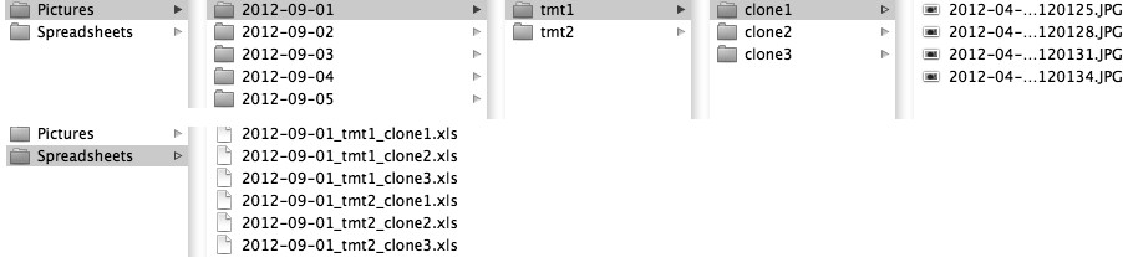
\includegraphics[width=0.95\textwidth]{2_Methodo/Fig/FigS1.pdf}
\caption[\lofimage{2_Methodo/Fig/FigS1.pdf}  Example of a directory tree and
resulting tables]{ Example of a directory tree with sorted pictures (upper part)
and the resulting tables (lower part).
}
\label{Fig21-S1}
\end{figure}

\begin{figure}[!ht] % Figure S2 
\centering
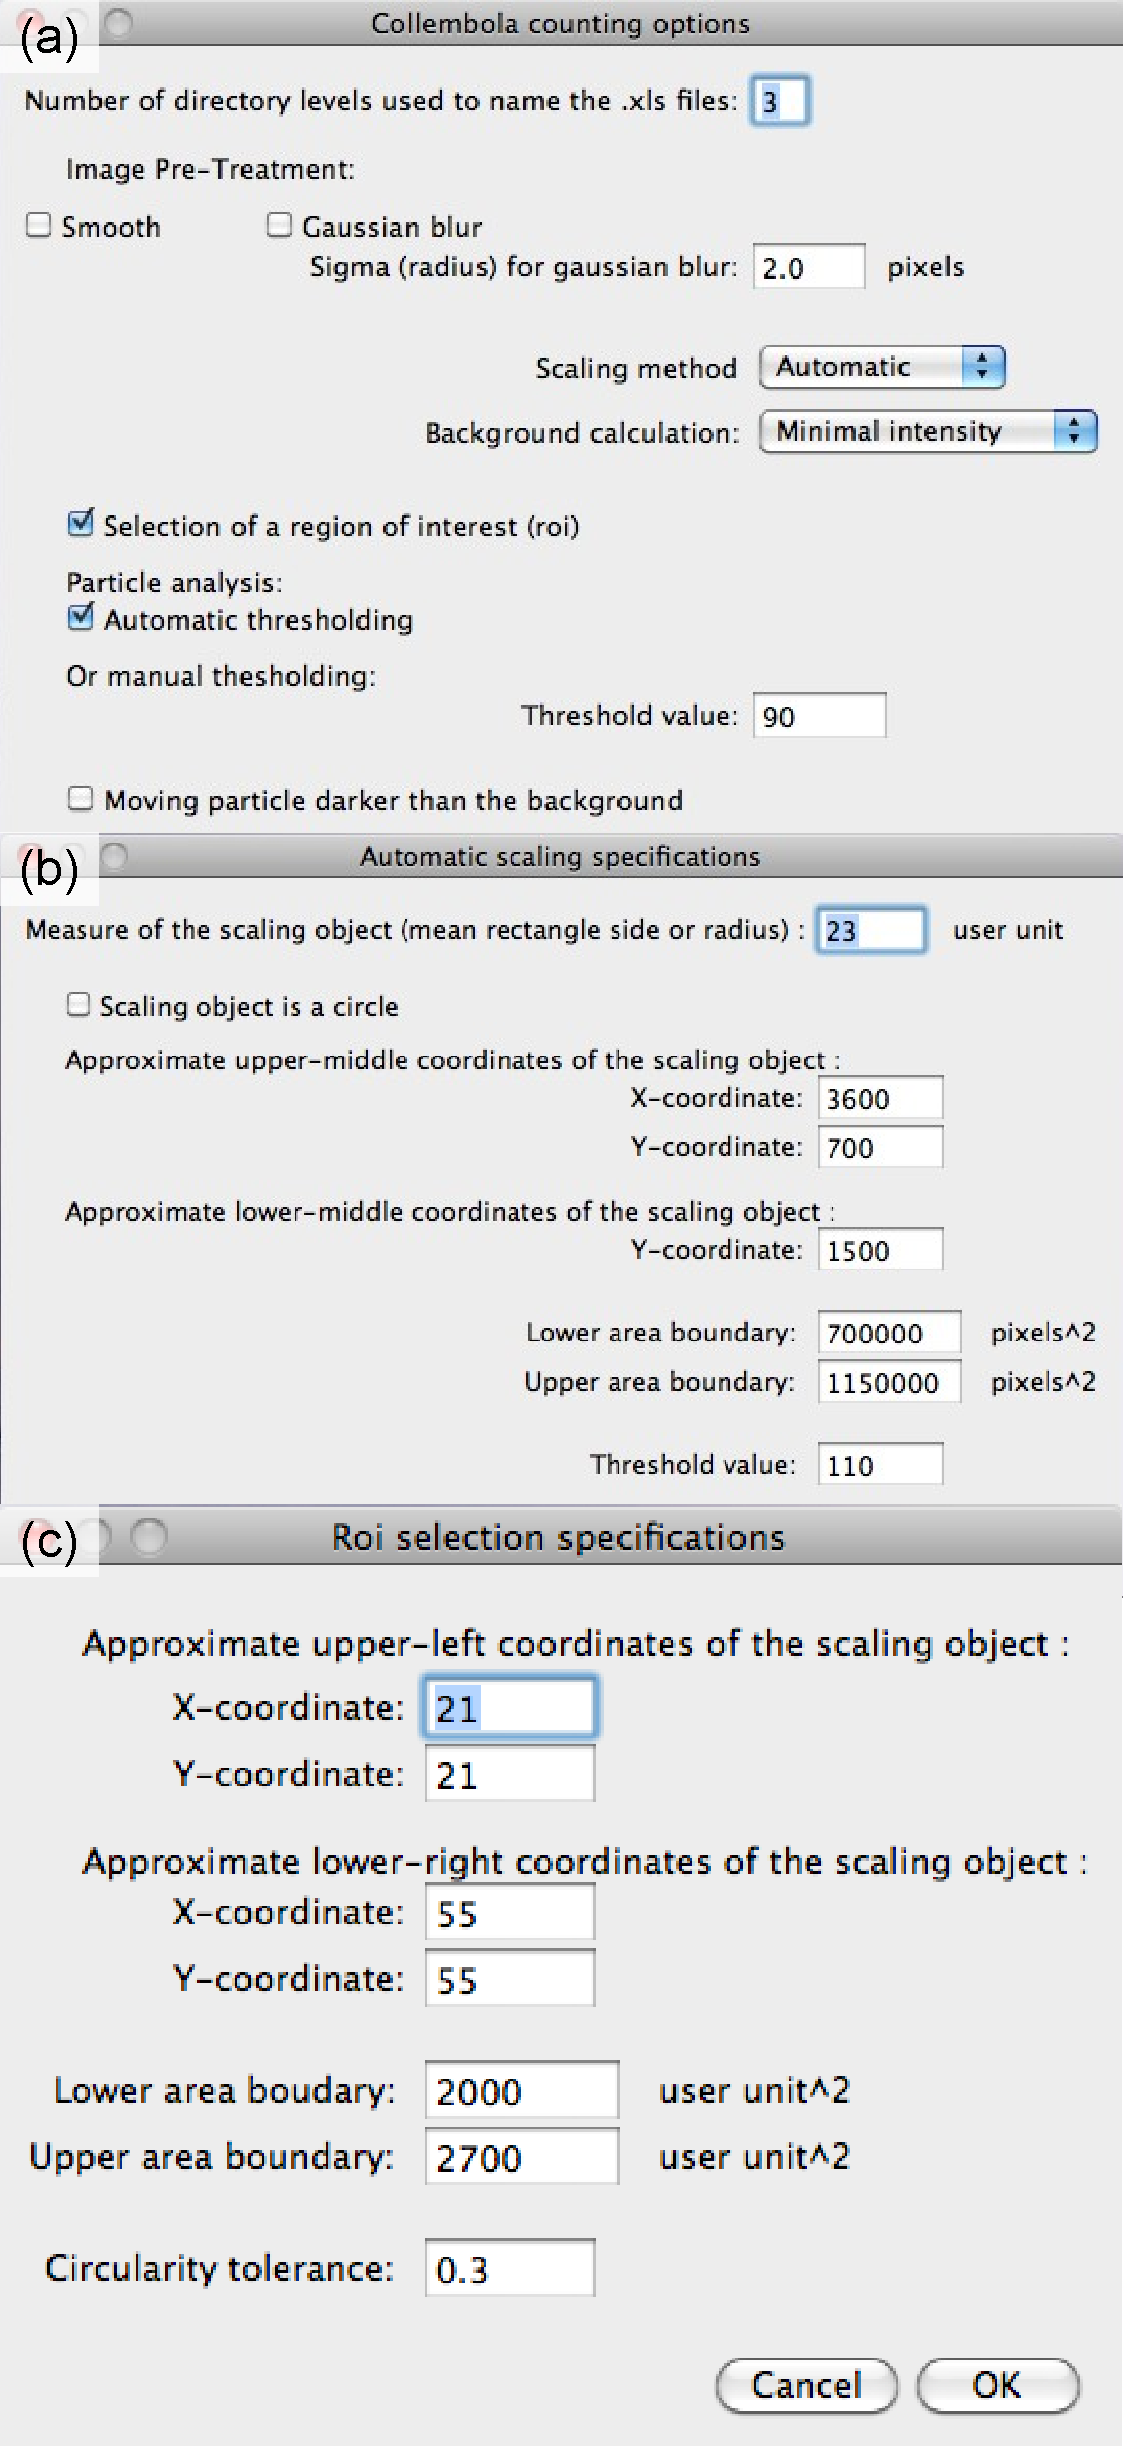
\includegraphics[height=0.85\textheight]{2_Methodo/Fig/FigS2.pdf}
\caption[\lofimage{2_Methodo/Fig/FigS2.pdf}  Plugin specification windows]{ Plugin specification windows. (a) On this window one is asked to specify the variables
described in Table 1. If selected, the automatic scaling specification window
(b) and the region of interest (roi) selection specifications window (c) will
open successively.
}
\label{Fig21-S2}
\end{figure}

As an example, we provide in the supporting material a set of pictures that can
be analysed with our plugin using the default values. The main steps are
illustrated in Figure \ref{Fig21-S3}: the background picture is first constructed (Figure
\ref{Fig21-S3}b) by comparing the different images in the stack (Figure
\ref{Fig21-S3}a), keeping only the minimal values (darker) for each pixel. This background picture is then
removed from the different images of the original stack. It creates a new stack
where only the moving particles remain (Figure \ref{Fig21-S3}d). In this example, the
background image is also used to scale the measurements. A black square on the
top right of the picture (arrow 2) is selected and measured to automatically
convert in mm the future measurements. It is also possible to select a reference
distance (arrow 1) to manually adjust the scale. The plugin will then detect the
boundary of the rearing box (Figure \ref{Fig21-S3}b, arrow 3), and retrieve on the new stack
of images this selected region of interest (Figure \ref{Fig21-S3}d). Within this boundary,
an automatic threshold is applied and the particles are measured and counted
(Figure \ref{Fig21-S3}d) The background removal is an essential step that makes possible the
automation of the thresholding. As shown in Figure \ref{Fig21-S3}, most of the substrate
heterogeneity is removed. Motionless particles or dead organisms are also
excluded from the automatic census (Figure \ref{Fig21-S3}, arrows 4 and 5). Without this
crucial step, a batch processing of large amounts of replicated populations
would not be possible and a threshold would have to be adjusted manually.

\begin{figure}[!ht] % Figure S3 
\centering
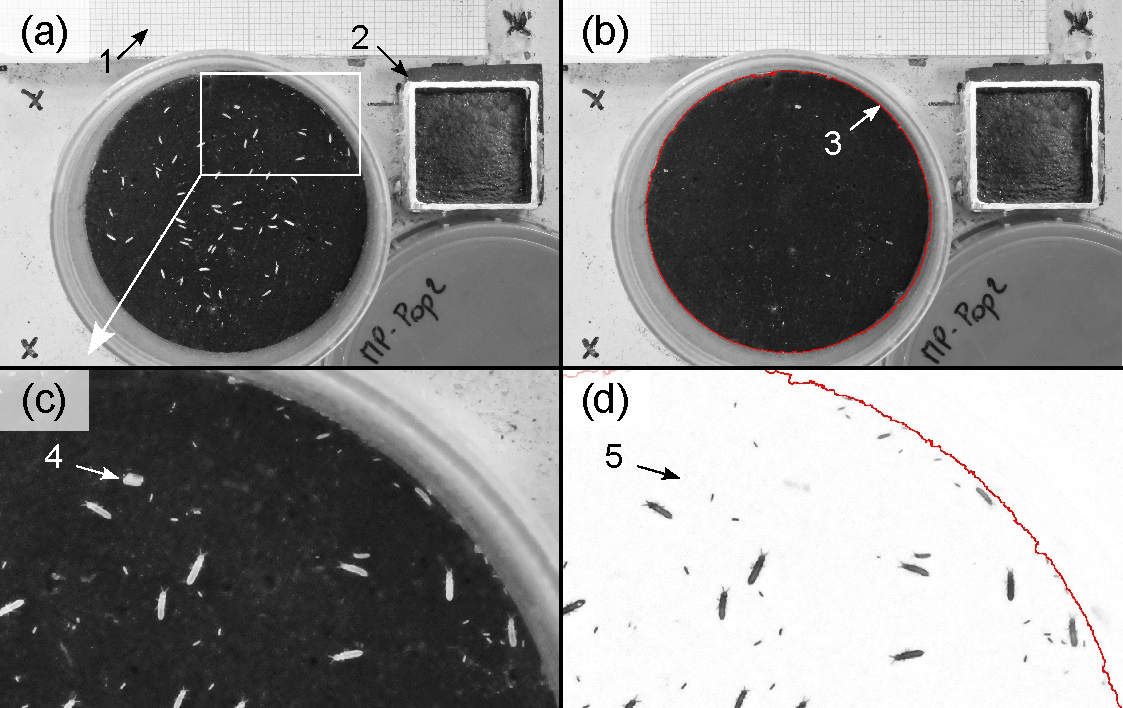
\includegraphics[width=0.95\textwidth]{2_Methodo/Fig/FigS3.pdf} 
\caption[\lofimage{2_Methodo/Fig/FigS3.pdf}Successive steps of the image processing]{
Successive steps of the image processing. (a) Original picture of a rearing box
with its collembola population. A piece of graph paper (arrow 1) and a
contrasted black square (arrow 2) can be used as references to scale the
measurements. (b) By comparing different images, a background picture is
generated: each pixel is the darker pixel of the original set of images. The
white moving collembola are automatically discarded. The border of the box
(arrow 3) is automatically detected and selected by the plugin. (c) Close-up
view of one of the original pictures. Arrow 4 points at a white dirt particle.
(d) Before analysing the particles within the region of interest, the plugin
removes the background which ensures measuring the moving particles only –
motionless white particles or reflections being automatically excluded from the
analysis (arrow 5).}
\label{Fig21-S3}
\end{figure}


Some parts of the provided java code can also be used separately: the automatic
scaling procedure can be used to speed up recursive manual size measurements on
pictures shot at various heights (for example, in field experiments without a
camera stand). One just has to add on each picture, at a relatively constant
position, a contrasted area that can be used for scaling.




\section{Acknowledgments}
We thank Lise Frézal and Marie-Anne Felix for providing the culture of
nematodes, David Carmignac for the \textit{Daphnia} and Romain Peronnet for the ant
colony.